\documentclass[10pt,tikz,border=1mm]{standalone} 
\usepackage{mathpazo}
\usepackage[T1]{fontenc}
\usetikzlibrary{positioning,calc,arrows.meta}
\tikzstyle{arrow}=[-{Stealth[scale=1.25]},thin,text=black,font=\normalsize,draw=black]
\tikzstyle{process}=[rectangle,minimum height=1.5cm,minimum width=2cm,fill=black!5,draw=black]
\tikzstyle{empty}=[circle,inner sep=0pt,fill=none]
\tikzstyle{hdist}=[node distance=2.5cm]
\tikzstyle{number}=[circle,fill=black!10,font=\footnotesize,inner sep=0.5mm,draw=black,thin]
\tikzstyle{arrow1}=[-{Stealth[scale=1.5]},thin,text=black,font=\normalsize,draw=black]
\begin{document}
	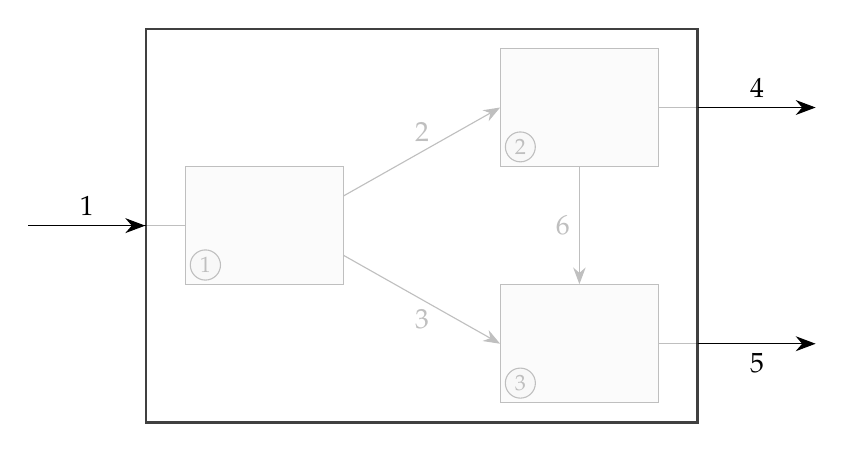
\begin{tikzpicture}
	%\draw[step=1cm,black!20,very thin] (-1,-2) grid (10,2);
	\node [empty] (V0)  {};
	\node [process] (N1) [right of=V0,hdist]{};
	\node [process,at={(6.5,1.5)}] (N2) {};
	\node [process,at={(6.5,-1.5)}] (N3) {};
	\node [empty] (W1) [right of=N2,hdist] {};
	\node [empty] (W2) [right of=N3,hdist] {};
	\draw (V0) -- (N1);
	\coordinate (N1a) at ($(N1.east)!0.5!(N1.north east)$);
	\coordinate (N1b) at ($(N1.east)!0.5!(N1.south east)$);
	\draw [arrow] (N1a) -- node[above]{2} (N2.west);
	\draw [arrow] (N1b) -- node[below]{3} (N3.west);
	\draw  (N2) -- (W1);
	\draw  (N3) -- (W2);
	\draw [arrow] (N2) -- node[left]{6} (N3);
	\node[number,at={(1.75,-0.5)}] {1};
	\node[number,at={(5.75,1)}] {2};
	\node[number,at={(5.75,-2)}] {3};
	\coordinate (D1) at (0.5,0);
	\coordinate (D2) at (0,1.5);
	\coordinate (A) at (0.75,0);
	\node (rect) at (4.5,0) [draw=black,thick,fill=white,nearly opaque,minimum width=7cm,minimum height=5cm] {};
	\draw[arrow1] ($(V0)-(D1)$) -- node[above]{1} (rect.west);
	\draw[arrow1] ($(rect.east)+(D2)$) -- node[above]{4} ($(W1)+(D1)$);
	\draw[arrow1] ($(rect.east)-(D2)$) -- node[below]{5}($(W2)+(D1)$);
	\end{tikzpicture}
\end{document}		
	